\documentclass[12pt,a4paper]{article}%
%Options -- Point size:  10pt (default), 11pt, 12pt
%        -- Paper size:  letterpaper (default), a4paper, a5paper, b5paper
%                        legalpaper, executivepaper
%        -- Orientation  (portrait is the default)
%                        landscape
%        -- Print size:  oneside (default), twoside
%        -- Quality      final(default), draft
%        -- Title page   notitlepage, titlepage(default)
%        -- Columns      onecolumn(default), twocolumn
%        -- Equation numbering (equation numbers on the right is the default)
%                        leqno
%        -- Displayed equations (centered is the default)
%                        fleqn (equations start at the same distance from the right side)
%        -- Open bibliography style (closed is the default)
%                        openbib
% For instance the command
%           \documentclass[a4paper,12pt,leqno]{article}
% ensures that the paper size is a4, the fonts are typeset at the size 12p
% and the equation numbers are on the left side
%====================Tabelas==============================================
\usepackage{multirow}
%=============================Símbolos Matemáticos=====================================================================
\usepackage{amsmath}
\usepackage{amsfonts}
\usepackage{amssymb}
%=======================================Figuras===========================================================
\usepackage{graphicx}
%\usepackage{wrapfig}
\usepackage{float}
%=====================================Língua e acentos=============================================================
\usepackage[brazil]{babel}
\usepackage[utf8]{inputenc}
\usepackage[T1]{fontenc}
%========================================Espaçamento==========================================================
\usepackage[top=3cm, bottom=2cm, left=2cm, right=2cm]{geometry}
\usepackage{indentfirst}
%=======================================Lista de códigos===========================================================
\usepackage{listings}                   % para formatar código-fonte
\lstset{numbers=left, numberstyle=\tiny, stepnumber=1, numbersep=5pt, basicstyle=\scriptsize , frame=trbl}
%======================================Latexdraw============================================================
%\usepackage[usenames,dvipsnames]{pstricks}
%\usepackage{epsfig}
%\usepackage{pst-grad} % For gradients
%\usepackage{pst-plot} % For axes
%==================================================================================================
%-------------------------------------------

\usepackage[numbers]{natbib}
\usepackage[numbib]{tocbibind}

\begin{document}

\begin{titlepage}
\begin{center}
\begin{figure}[h]

\includegraphics[scale=0.76]{Imagens/topdotitulo.png}
\end{figure}
\rule{\columnwidth}{1.5mm}
\

\large David Maykon Krepsky Silva\\
\large Havena Louise Pavão

\vspace{4cm}
{\bf \Large Título do Experimento}
\vspace{3.5cm}

\begin{flushright}
Data de realização do experimento:\\
XX de abril de 2016\\
Série/Turma:\\
1000/1011\\
Prof. Me. Jaime Laelson Jacob 
\end{flushright}

\vspace{3.2cm}
\today

\rule{\columnwidth}{1.3mm}
\end{center}
\end{titlepage}
\newpage

\begin{abstract}
\addcontentsline{toc}{section}{Resumo}

Neste trabalho foi realizado o estudo de filtros passivos compostos indutores e 
capacitores (filtros LC) de forma a analisar a resposta em frequência para 
filtro passa baixas (FPB), filtro passa alta (FPA) e filtro passa faixa (FPF). 
A metodologia utilizada consiste em realizar o projeto do filtro normalizado, 
transformar para o tipo de filtro requerido e simular o circuito no software 
Orcad.
Durante o laboratório foi possível observar as diferentes respostas em frequência para cada tipo de filtro estudado.Também foi visualizado a melhora no fator Q de filtros em cascata em relação a um único filtro de ordem mais alta.
\end{abstract}
\newpage

\tableofcontents

\newpage

\section{Introdução}
Explique qual a proposta do experimento. Situe seu trabalho no tempo e no espaço. Se quiser, mostre um breve (muito breve) esboço histórico do problema. Mostre resumidamente sua relevância para a comunidade a que é endereçado. Mostre sua utilidade (em que área é usado). Se possível, situe o problema em relação a outras áreas as quais está relacionado. Deixe claros os objetivos do trabalho.


\newpage

\section{Teoria}
Frequentemente em física, uma experiência é executada para testar uma teoria ou aproximações dela decorrentes. Enfim, para testar um modelo. Outras vezes, utiliza-se uma teoria já suficientemente testada tendo em vista uma aplicação. Nesta parte, você deve colocar os resultados teóricos que são relevantes para o trabalho. Em geral, não são feitas deduções, mas os aspectos da teoria utilizada (relações matemáticas, afirmações etc) são discutidos. Deixe claro o que é cada grandeza utilizada e o significado físico das relações usadas. Neste item, você deve fazer uso de referências onde a teoria foi desenvolvida (livros, apostilas, relatórios, artigos etc).

\newpage

\section{Metodologia Experimental}

Este experimento foi dividido em 4 circuitos, o qual foram projetados utilizando a tabela de coeficientes normalizados provida pelo professor e, em seguida, foram simulados no programa computacional Cadence Orcad. Abaixo segue a descrição de cada circuito.

\subsection{FPB}
O primeiro filtro projetado foi um filtro passa-baixas de terceira ordem, com resposta do tipo Butterworth utilizando apenas 1 indutor. A frequência de corte dada é de 4,8 kHz, o resistor da fonte $R_s = 50\ \Omega$ e a carga $R_l = 470\ \Omega$.

Foram analisadas a frequência de corte, atenuação fora da faixa de passagem, atenuação na faixa de passagem e a defasagem ao longo de toda a faixa de frequências.

A figura \ref{fFPB} mostra o circuito utilizado.\begin{figure}[H]
    \centering
    
    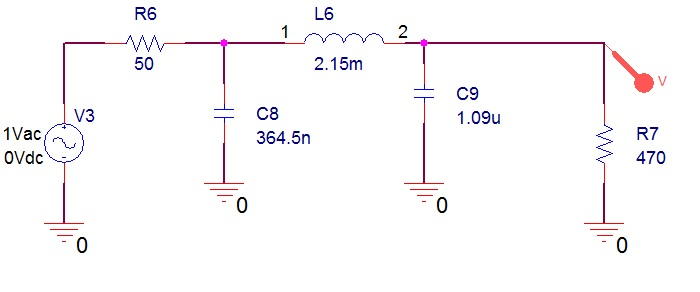
\includegraphics[scale=0.8]{Imagens/fpb.jpg}
    \label{fFPB}
    \caption{Filtro desnormalizado passa-baixas.}
\end{figure}



\subsection{FPA}
O segundo filtro projetado foi um filtro passa-altas de terceira ordem, com resposta do tipo Butterworth utilizando apenas 1 indutor. A frequência de corte dada é de 4,2 kHz, o resistor da fonte $R_s = 470 \Omega$ e a carga $R_l = 50 \Omega$.

Foram analisadas a frequência de corte, atenuação fora da faixa de passagem, atenuação na faixa de passagem e a defasagem ao longo de toda a faixa de frequências.

A figura \ref{fFPA} mostra o circuito utilizado.\begin{figure}[H]
    \centering
    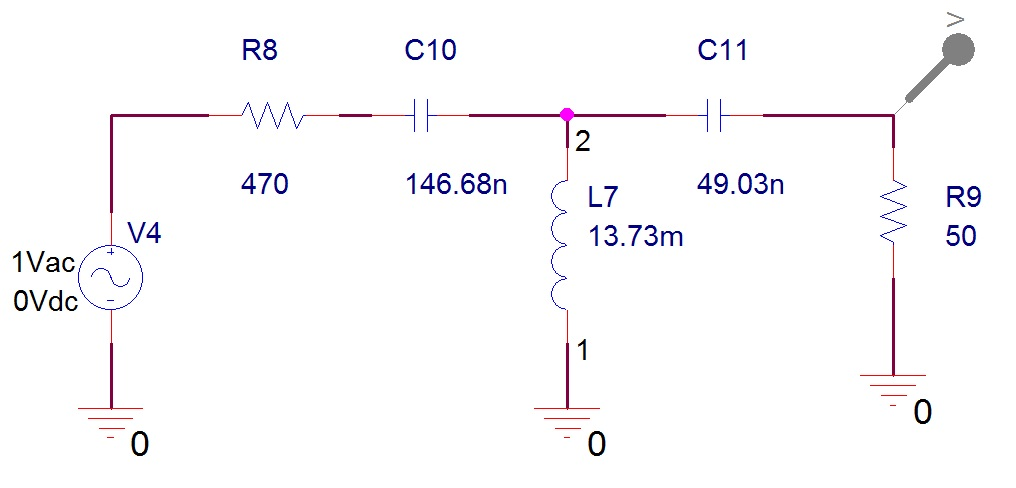
\includegraphics[scale=0.5]{Imagens/fpa.jpg}
    \label{fFPA}
    \caption{Filtro desnormalizado passa-altas.}
\end{figure}

\subsection{FPF em cascata}
No terceiro circuito o filtro FPB e o FPA desenvolvidos anteriormente foram conectados em cascata de forma a formar um filtro passa-faixa, onde foi também analisado a largura de banda passante do filtro.

Na figura \ref{fFPFC} é apresentado o circuito resultante da conexão dos filtro FPA e FPB, na topologia cascata.

\begin{figure}[H]
    \centering
    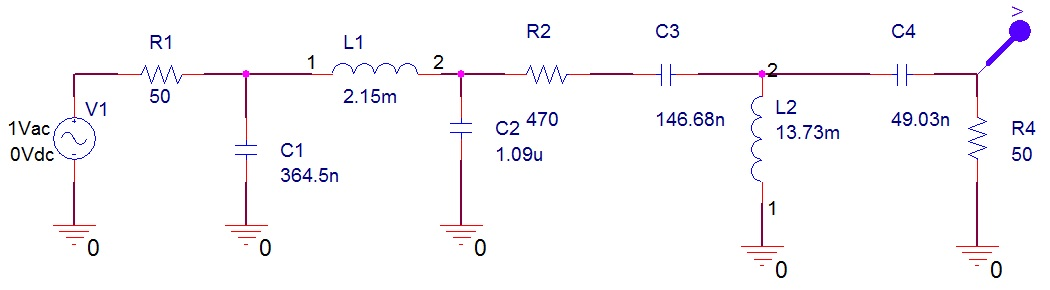
\includegraphics[scale=0.5]{Imagens/fpf1.jpg}
    \label{fFPFC}
    \caption{Filtro passa-faixa em cascata.}
\end{figure}

\subsection{FPF}
O quarto e ultimo filtro foi projetado para ter uma resposta em frequência semelhante a do filtro FPF em cascata. O objetivo foi de analisar as diferenças em se utilizar um filtro FPF e um filtro FPB em conjunto com um filtro FPA.

A figura \ref{fFPF} representa o filtro passa-faixa projetado.

\begin{figure}[H]
    \centering
    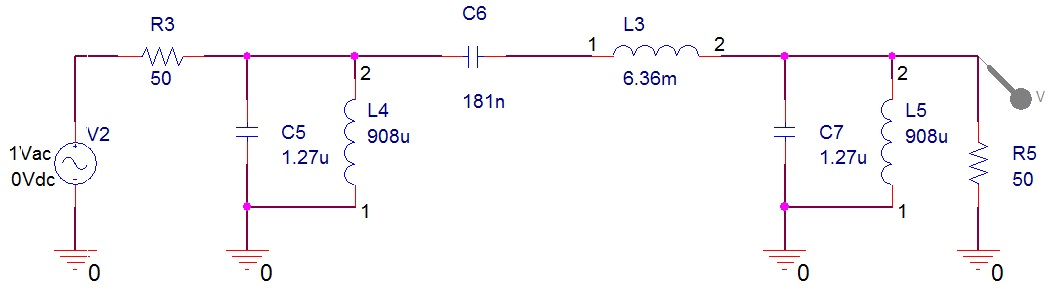
\includegraphics[scale=0.5]{Imagens/fpf2.jpg}
    \label{fFPF}
    \caption{Filtro passa-faixa.}
\end{figure}

\newpage

\section{Resultados e Análise de Dados}

\subsection{FPB}
O primeiro filtro projetado foi um filtro passa-baixas de terceira ordem, com 
resposta do tipo Butterworth utilizando apenas 1 indutor.

A figura \ref{fig:fpb-norm} mostra o circuito normalizado.
\begin{figure}[!h]
  \centering
  
  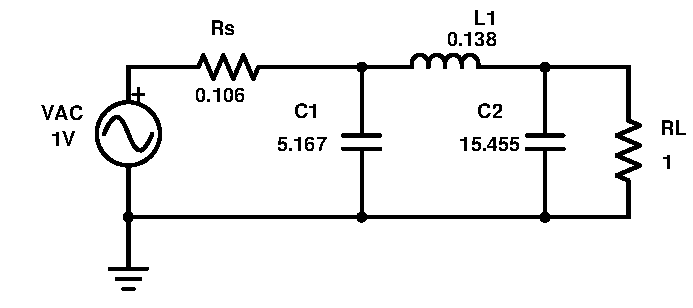
\includegraphics[scale=0.4]{Imagens/fpb-norm}
  \label{fig:fpb-norm}
  \caption{Filtro passa-baixas normalizado.}
\end{figure}


A figura \ref{fig:fpb} mostra o circuito já desnormalizado, pronto para 
simulação.
\begin{figure}[!h]
  \centering
  
  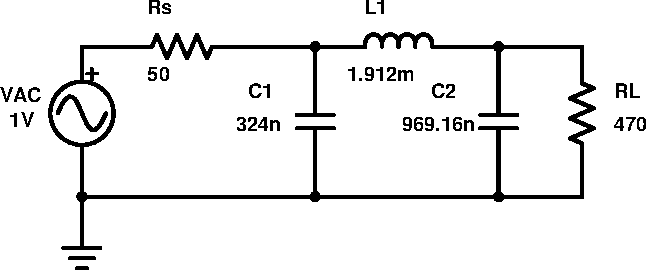
\includegraphics[scale=0.4]{Imagens/fpb}
  \label{fig:fpb}
  \caption{Filtro desnormalizado passa-baixas.}
\end{figure}

A resposta em frequência obtida está na figura \ref{fig:resp_freq}, onde foi 
obtido uma frequência de corte de 5,317 kHz. 

\begin{figure}[!h]
  \centering
  
  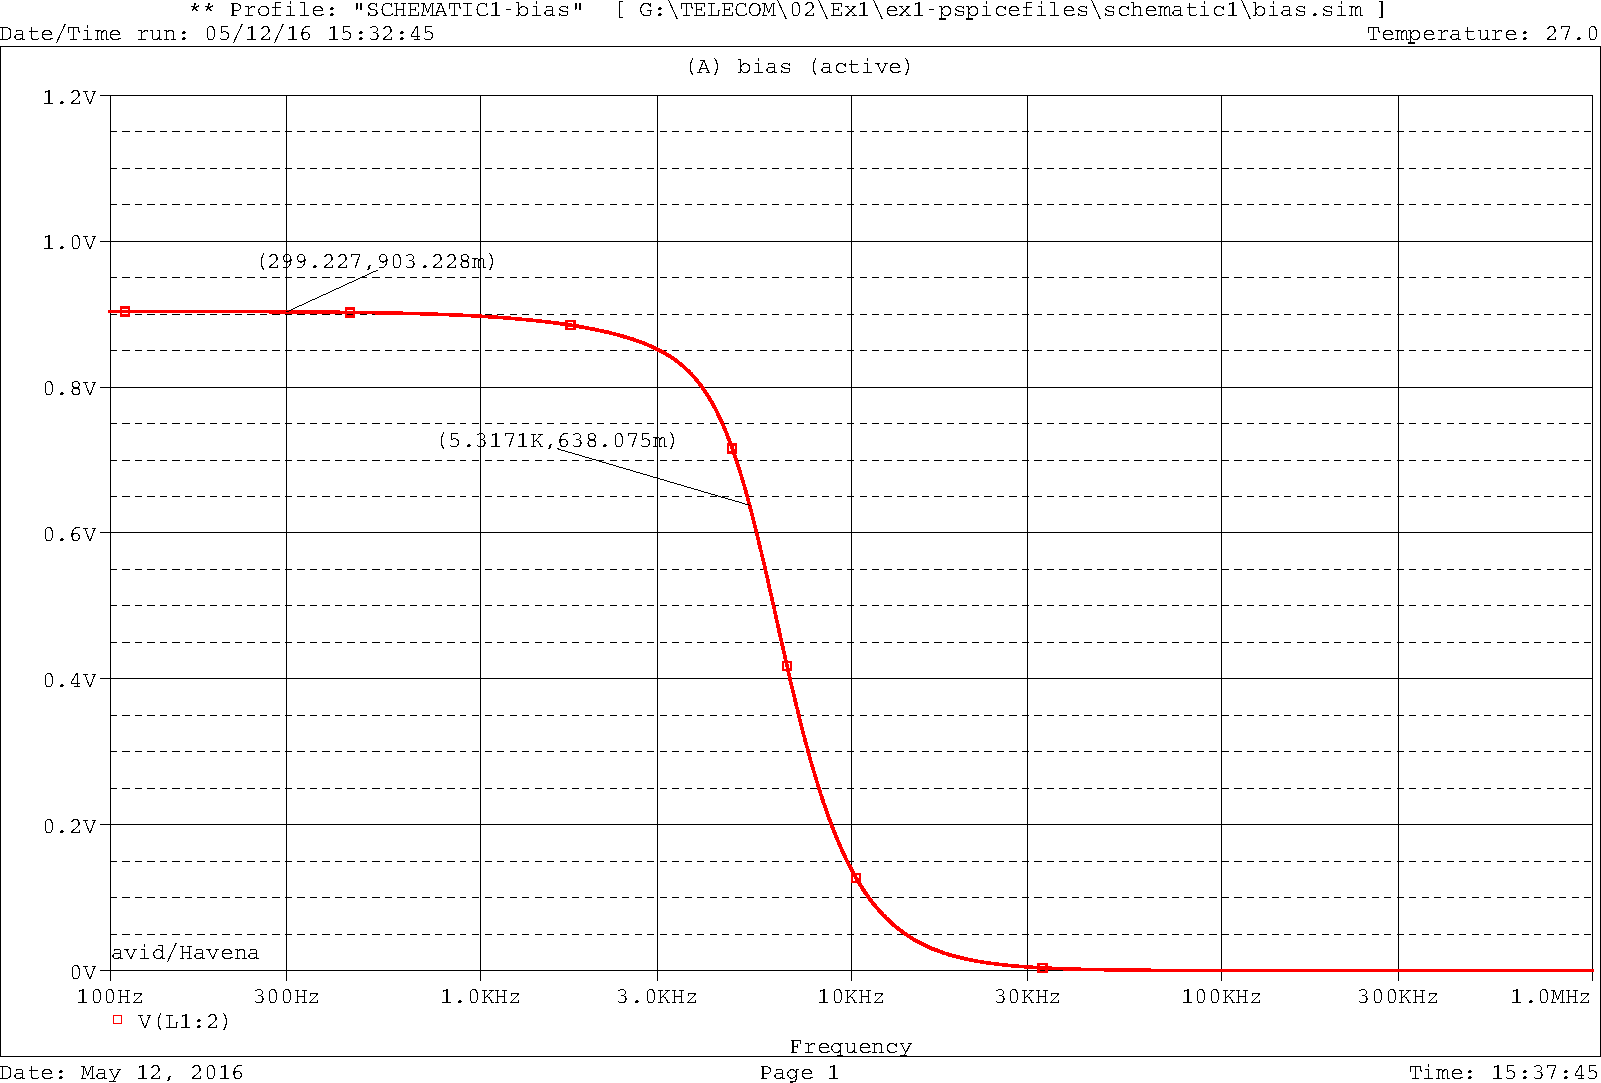
\includegraphics[scale=0.3]{Imagens/resp_freq}
  \label{fig:resp_freq}
  \caption{Resposta em frequência do filtro passa-baixas.}
\end{figure}

A figura \ref{fig:resp_freq_db} mostra a resposta em dB, nota-se que a 
atenuação aumenta em aproximadamente 60 dB por década, o que corresponde a 
ordem 3 do filtro.

\begin{figure}[!h]
  \centering
  
  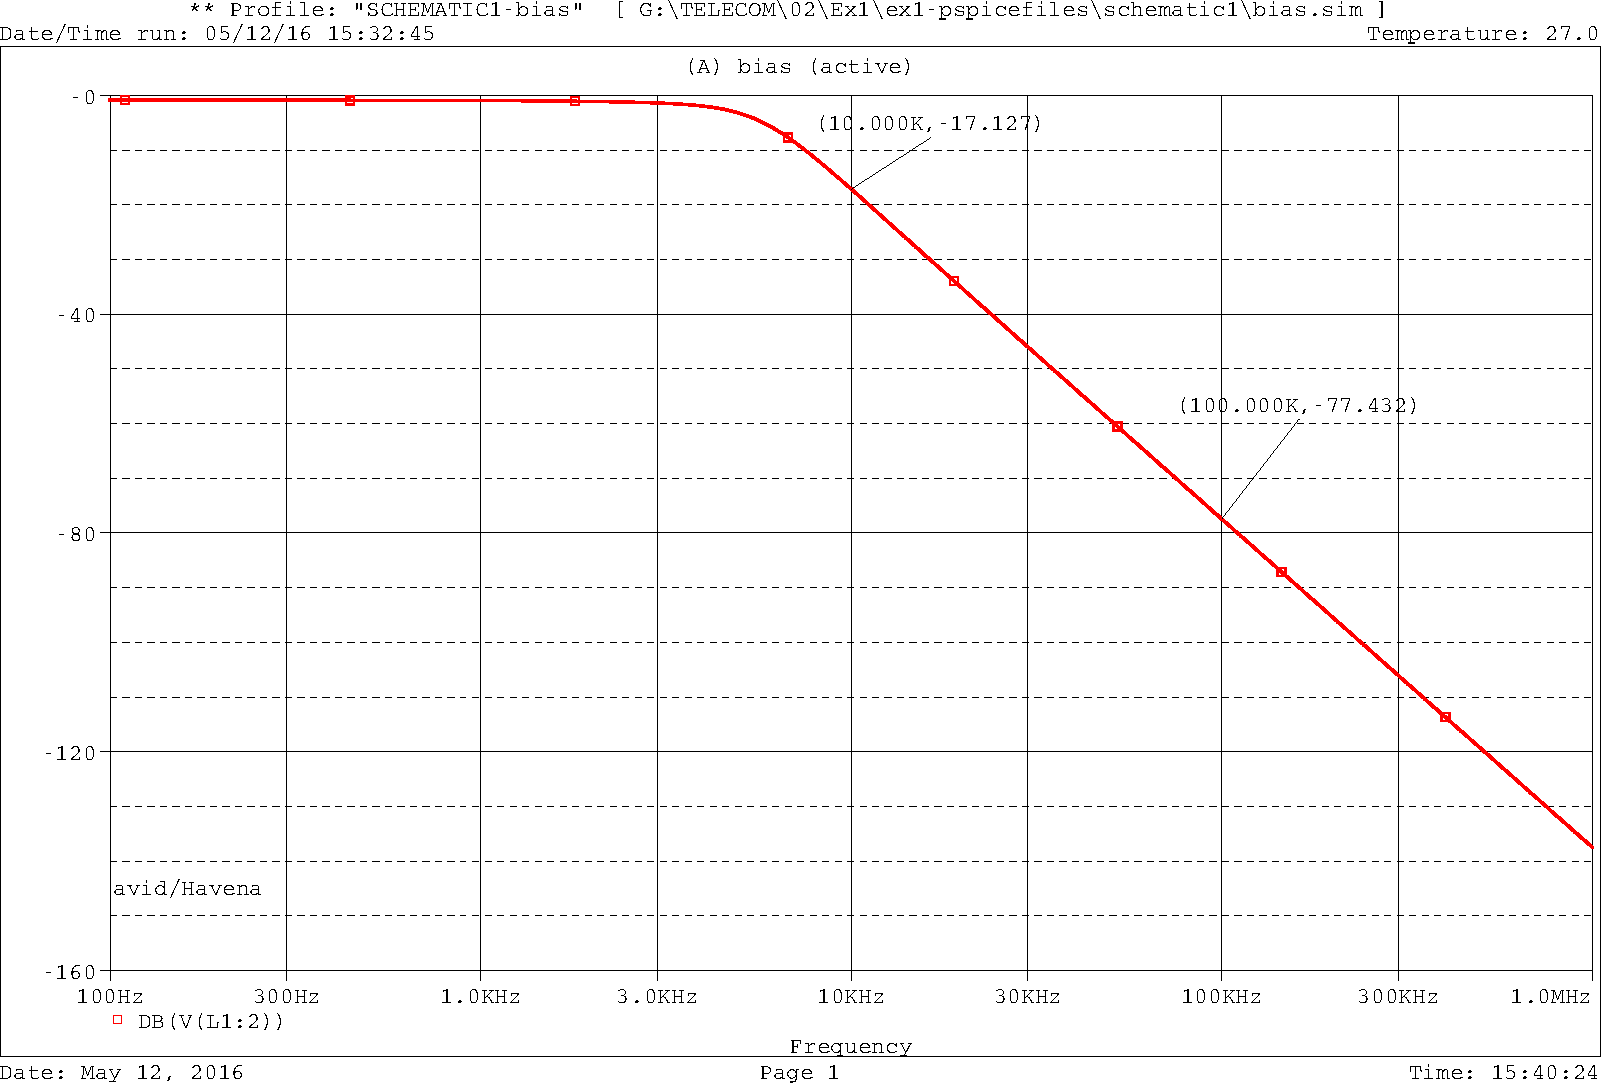
\includegraphics[scale=0.3]{Imagens/resp_freq_db}
  \label{fig:resp_freq_db}
  \caption{Resposta em frequência do filtro passa-baixas em dB.}
\end{figure}

A figura \ref{fig:resp_freq_phase} mostra a fase da resposta em frequência para 
o filtro passa baixas, onde é possível observar uma defasagem de 270 graus, o 
que condiz com a teoria pois o filtro é de ordem 3.

\begin{figure}[!h]
  \centering
  
  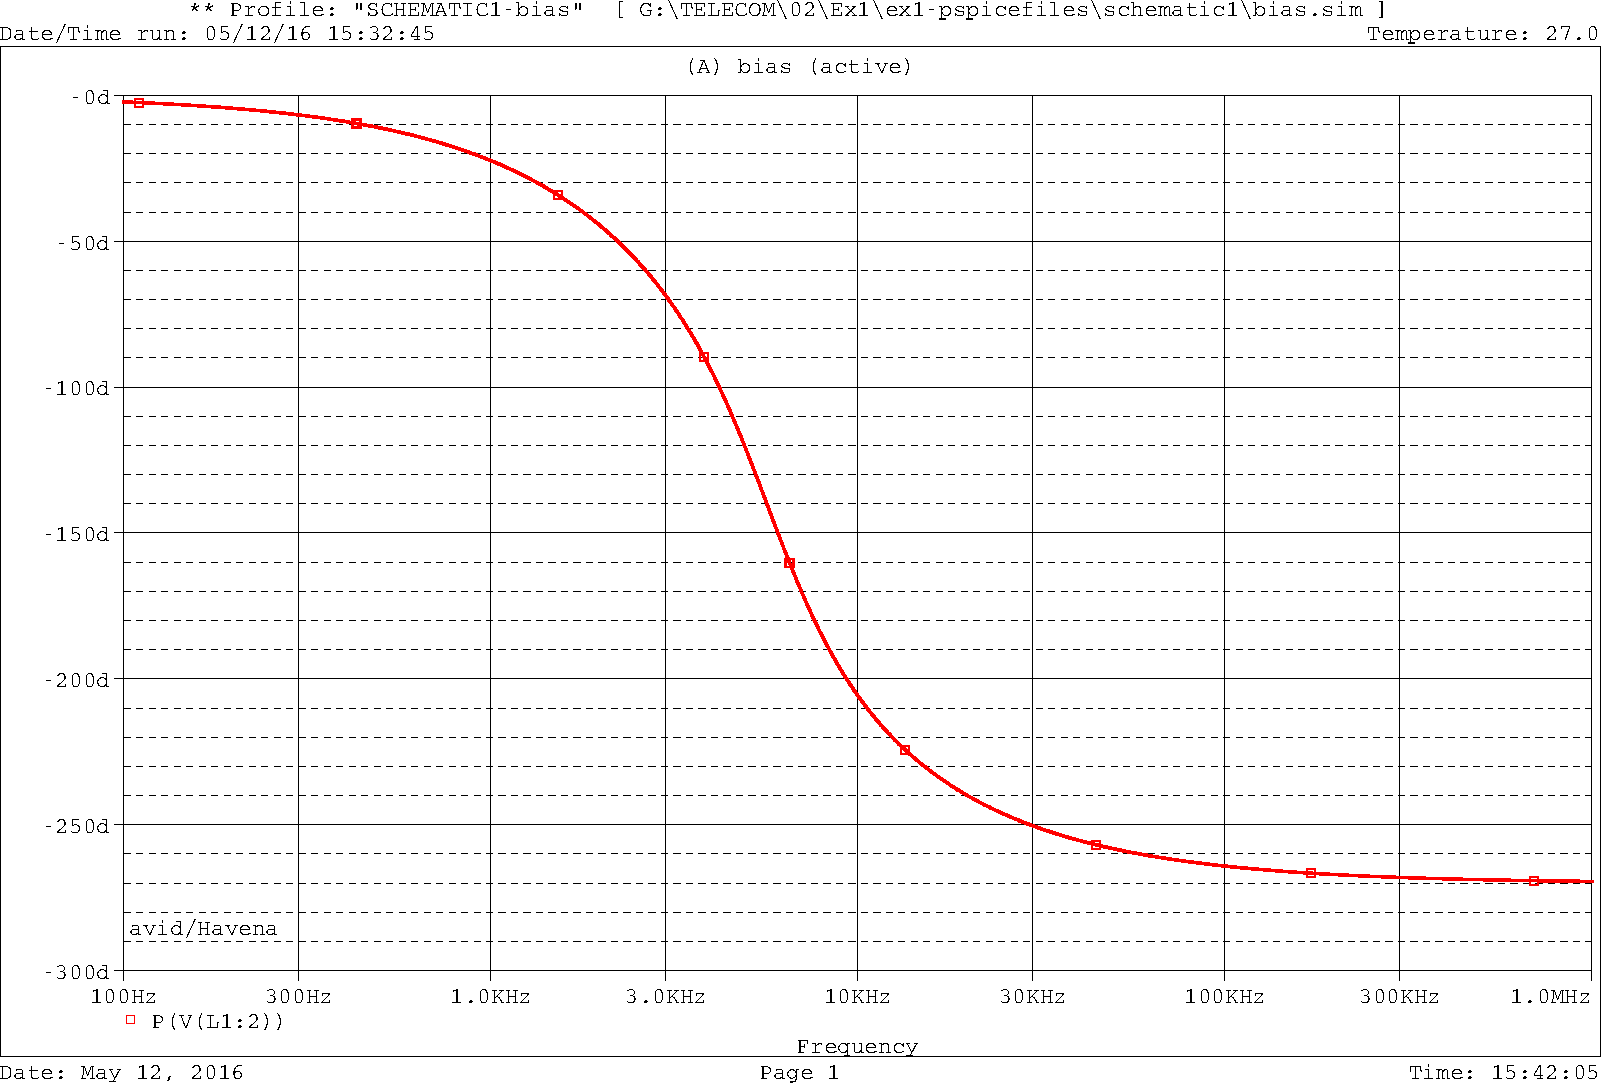
\includegraphics[scale=0.3]{Imagens/resp_freq_phase}
  \label{fig:resp_freq_phase}
  \caption{Fase da resposta em frequência do filtro passa-baixas.}
\end{figure}

\subsection{FPA}
O segundo filtro projetado foi um filtro passa-altas de terceira ordem, com 
resposta do tipo Butterworth utilizando apenas 1 indutor.

A figura \ref{fig:fpa-norm} mostra o circuito normalizado.
\begin{figure}[!h]
  \centering
  
  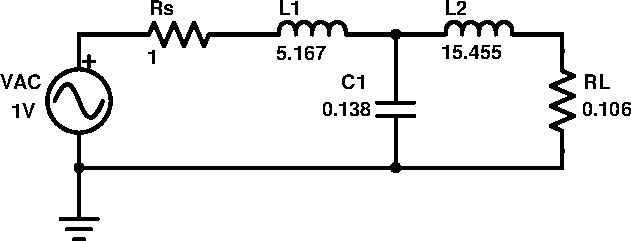
\includegraphics[scale=0.4]{Imagens/fpa-norm}
  \label{fig:fpa-norm}
  \caption{Filtro passa-altas normalizado.}
\end{figure}

A figura \ref{fig:fpa} mostra o circuito já desnormalizado, pronto para 
simulação.

\begin{figure}[!h]
  \centering
  
  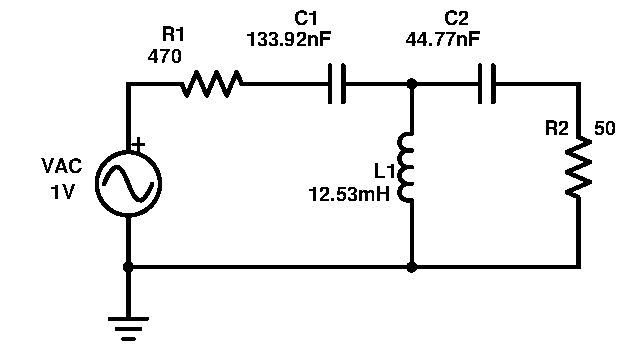
\includegraphics[scale=0.4]{Imagens/fpa}
  \label{fig:fpa}
  \caption{Filtro desnormalizado passa-altas.}
\end{figure}

A resposta em frequência obtida está na figura \ref{fig:resp_freq_2}, onde foi 
obtido uma frequência de corte de 4,384 kHz. 

\begin{figure}[!h]
  \centering
  
  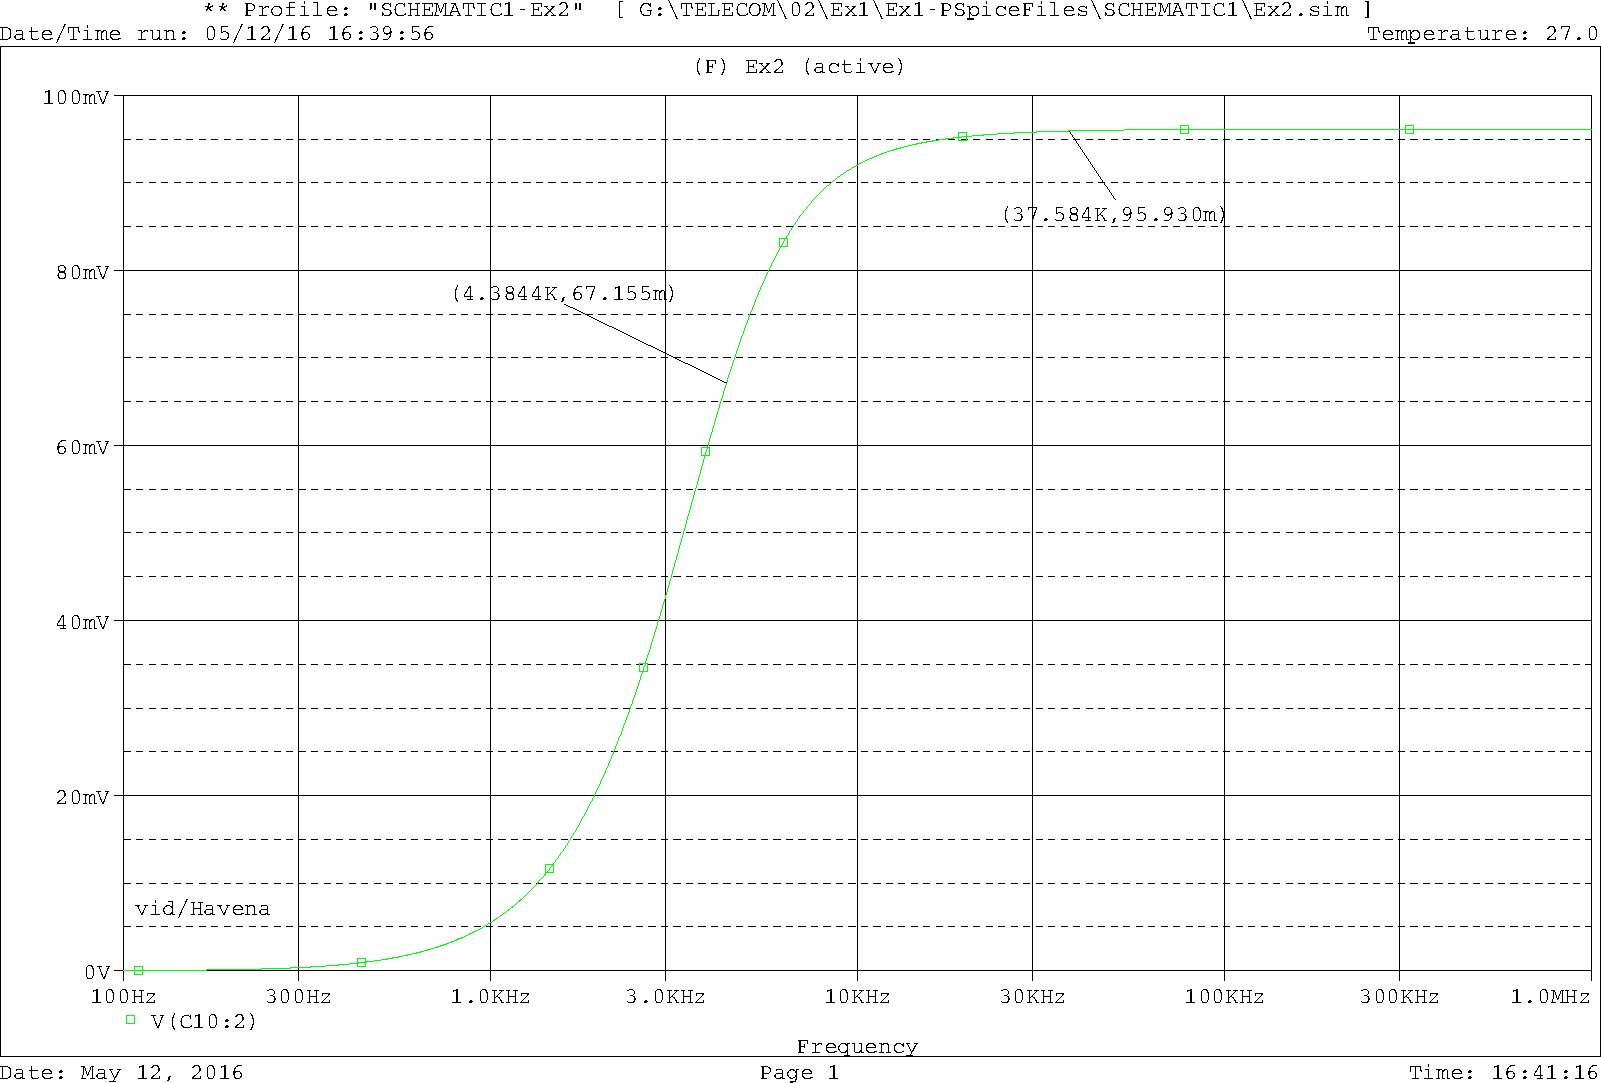
\includegraphics[scale=0.3]{Imagens/resp_freq_2}
  \label{fig:resp_freq_2}
  \caption{Resposta em frequência do filtro passa-altas.}
\end{figure}

A figura \ref{fig:resp_freq_db_2} mostra a resposta em dB, nota-se que a 
atenuação aumenta em aproximadamente 60 dB por década, o que corresponde a 
ordem 3 do filtro.

\begin{figure}[!h]
  \centering
  
  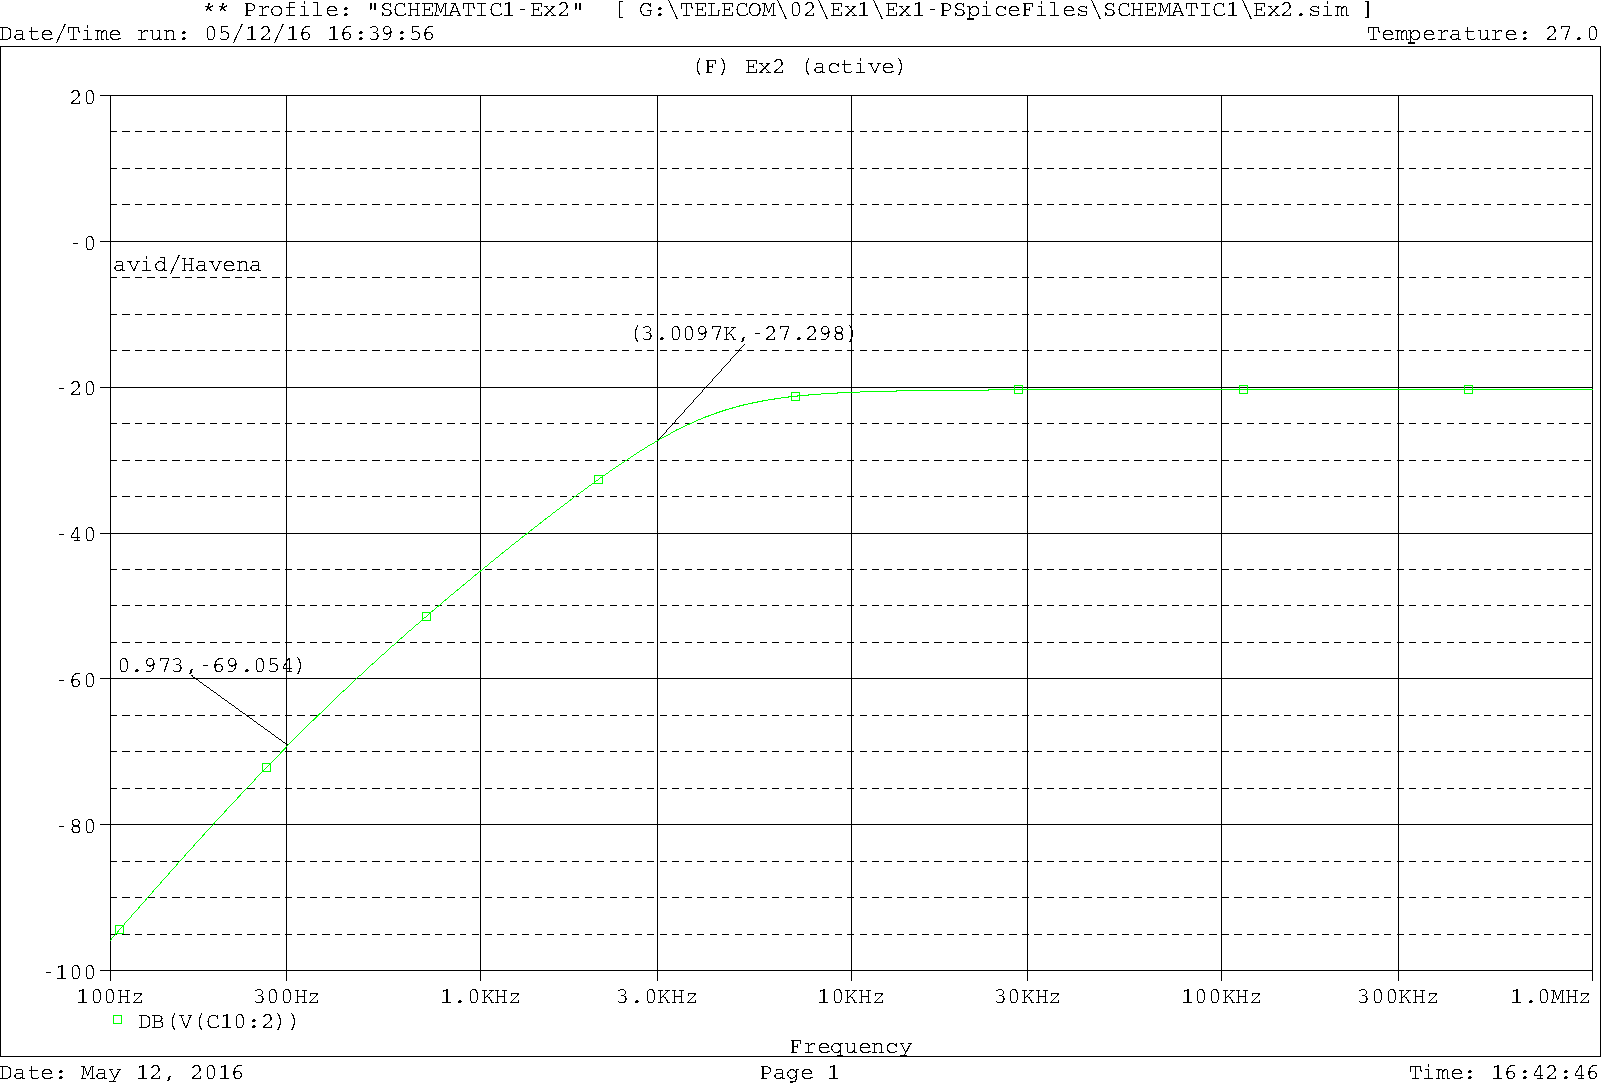
\includegraphics[scale=0.3]{Imagens/resp_freq_db_2}
  \label{fig:resp_freq_db_2}
  \caption{Resposta em frequência do filtro passa-altas em dB.}
\end{figure}

A figura \ref{fig:resp_freq_phase_2} mostra a fase da resposta em frequência 
para o filtro passa altas, onde é possível observar uma defasagem de 270 graus, 
o que condiz com a teoria pois o filtro é de ordem 3.

\begin{figure}[!h]
  \centering
  
  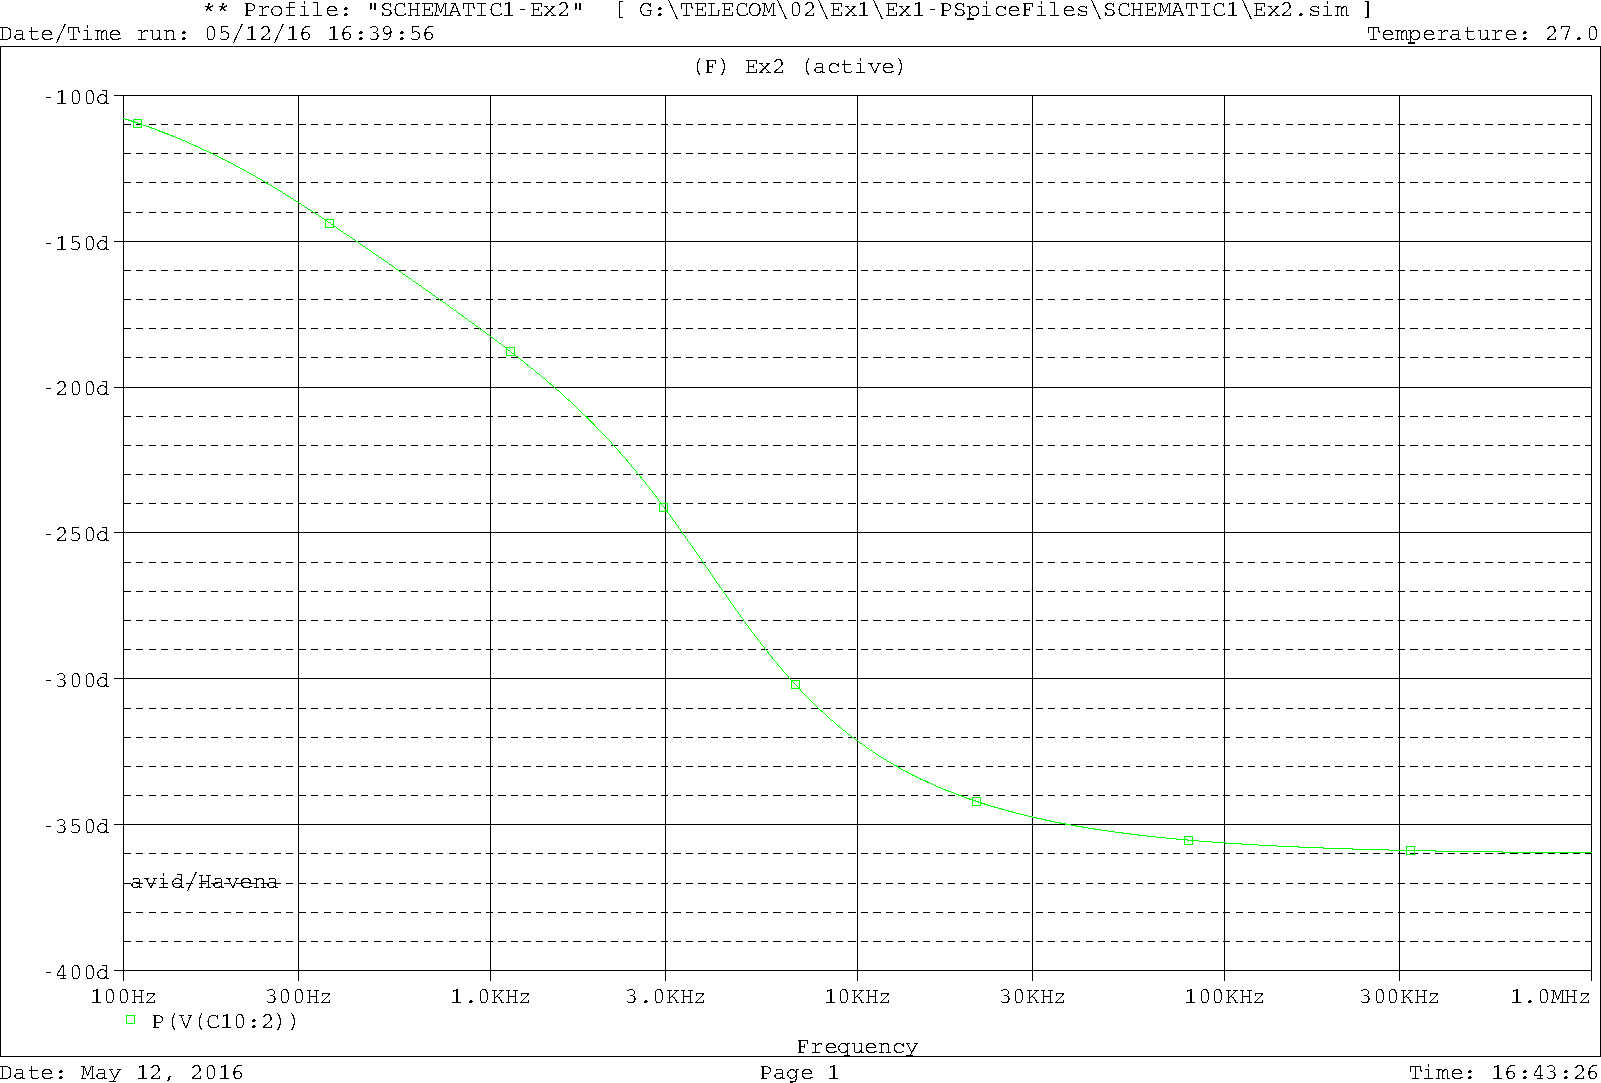
\includegraphics[scale=0.3]{Imagens/resp_freq_phase_2}
  \label{fig:resp_freq_phase_2}
  \caption{Fase da resposta em frequência do filtro passa-altas.}
\end{figure}

\subsection{FPF em cascata}
O terceiro filtro projetado foi um filtro passa-faixas em cascata de terceira 
ordem, com resposta do tipo Butterworth utilizando apenas 1 indutor.

A figura \ref{fig:fpf-cascata} mostra o circuito já desnormalizado, pronto para 
simulação.

\begin{figure}[!h]
  \centering
  
  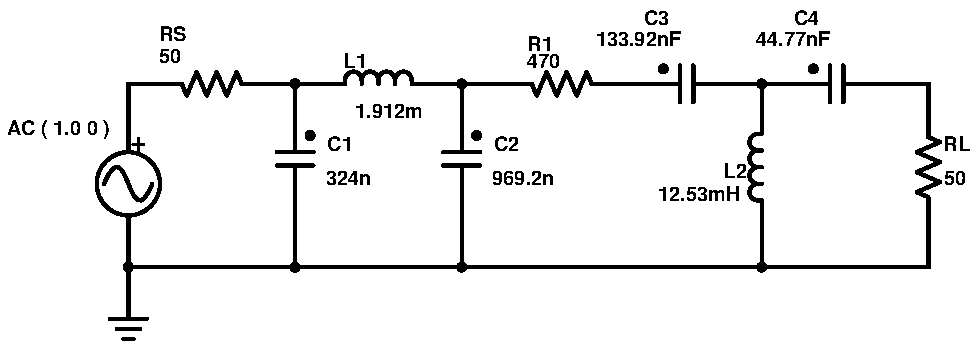
\includegraphics[scale=0.4]{Imagens/fpf-cascata}
  \label{fig:fpf-cascata}
  \caption{Filtro desnormalizado passa-faixa em cascata.}
\end{figure}

A resposta em frequência obtida está na figura \ref{fig:resp_freq_3}, onde foi 
obtido uma frequência central de 4,655 kHz. 

\begin{figure}[!h]
  \centering
  
  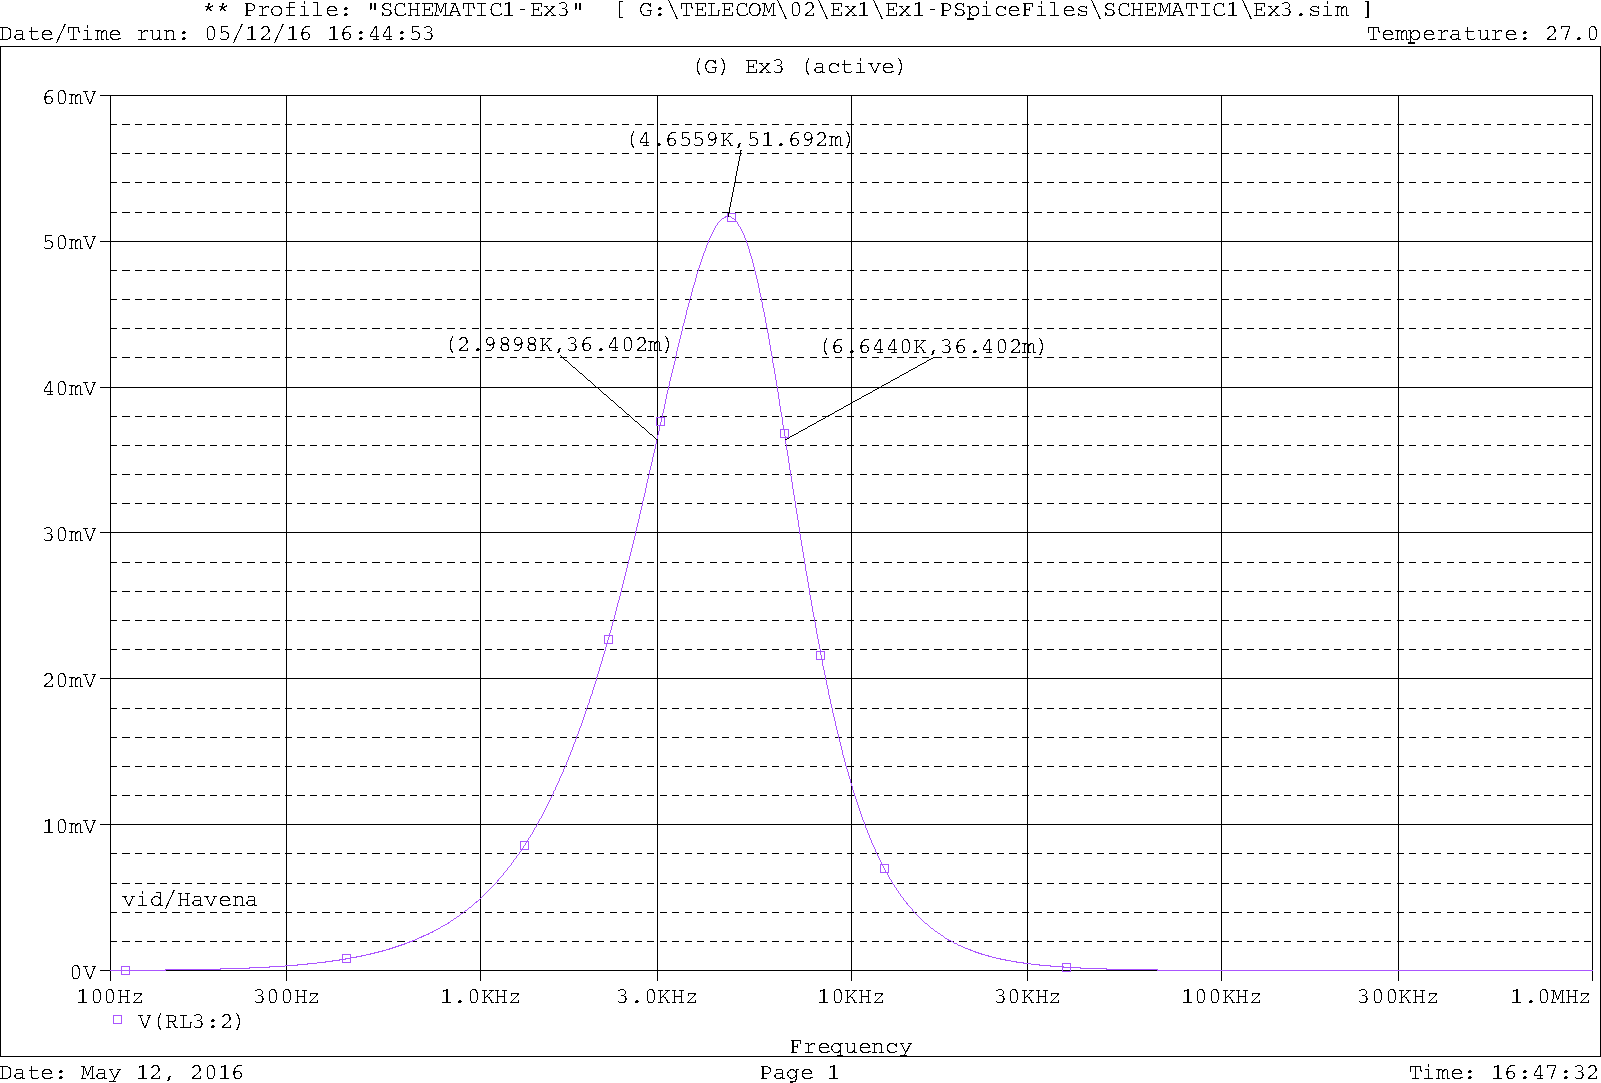
\includegraphics[scale=0.3]{Imagens/resp_freq_3}
  \label{fig:resp_freq_3}
  \caption{Resposta em frequência do filtro passa-faixa em cascata.}
\end{figure}

A figura \ref{fig:resp_freq_db_3} mostra a resposta em dB, nota-se que a 
atenuação aumenta em aproximadamente 60 dB por década, o que corresponde a 
ordem 3 do filtro.

\begin{figure}[!h]
  \centering
  
  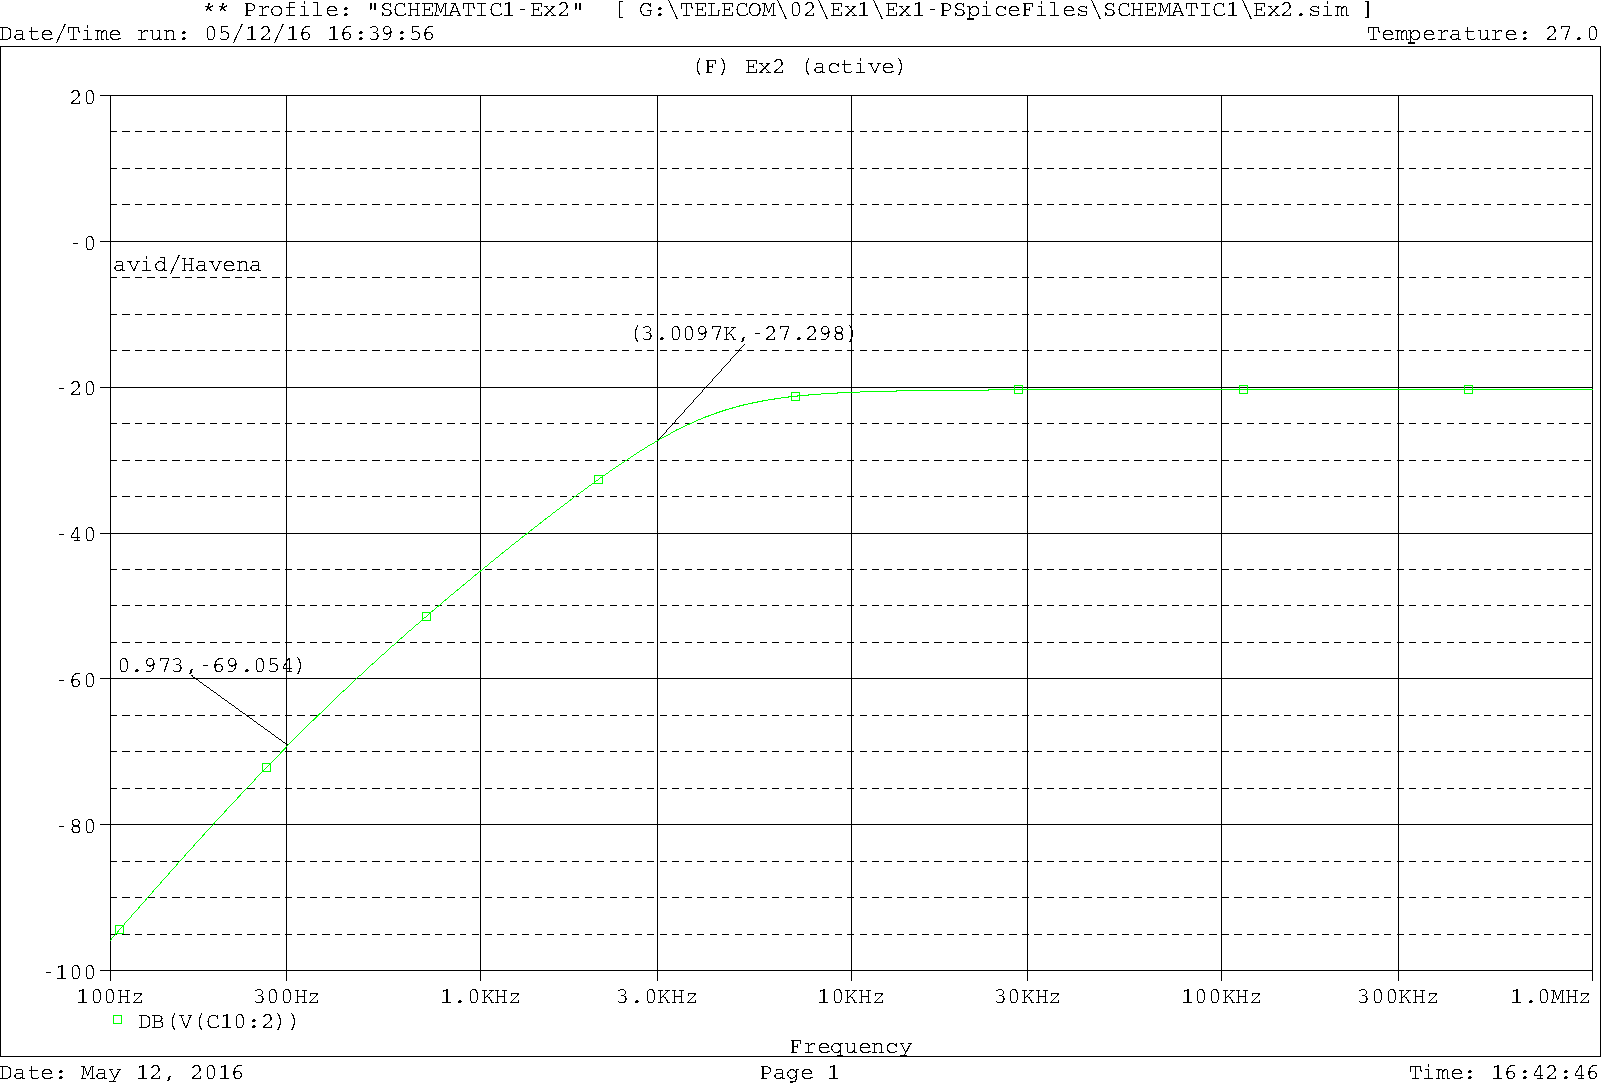
\includegraphics[scale=0.3]{Imagens/resp_freq_db_2}
  \label{fig:resp_freq_db_3}
  \caption{Resposta em frequência do filtro passa-faixa em cascata em dB.}
\end{figure}

A figura \ref{fig:resp_freq_phase_3} mostra a fase da resposta em frequência 
para o filtro passa altas, onde é possível observar uma defasagem de 270 graus, 
o que condiz com a teoria pois o filtro é de ordem 3.

\begin{figure}[!h]
  \centering
  
  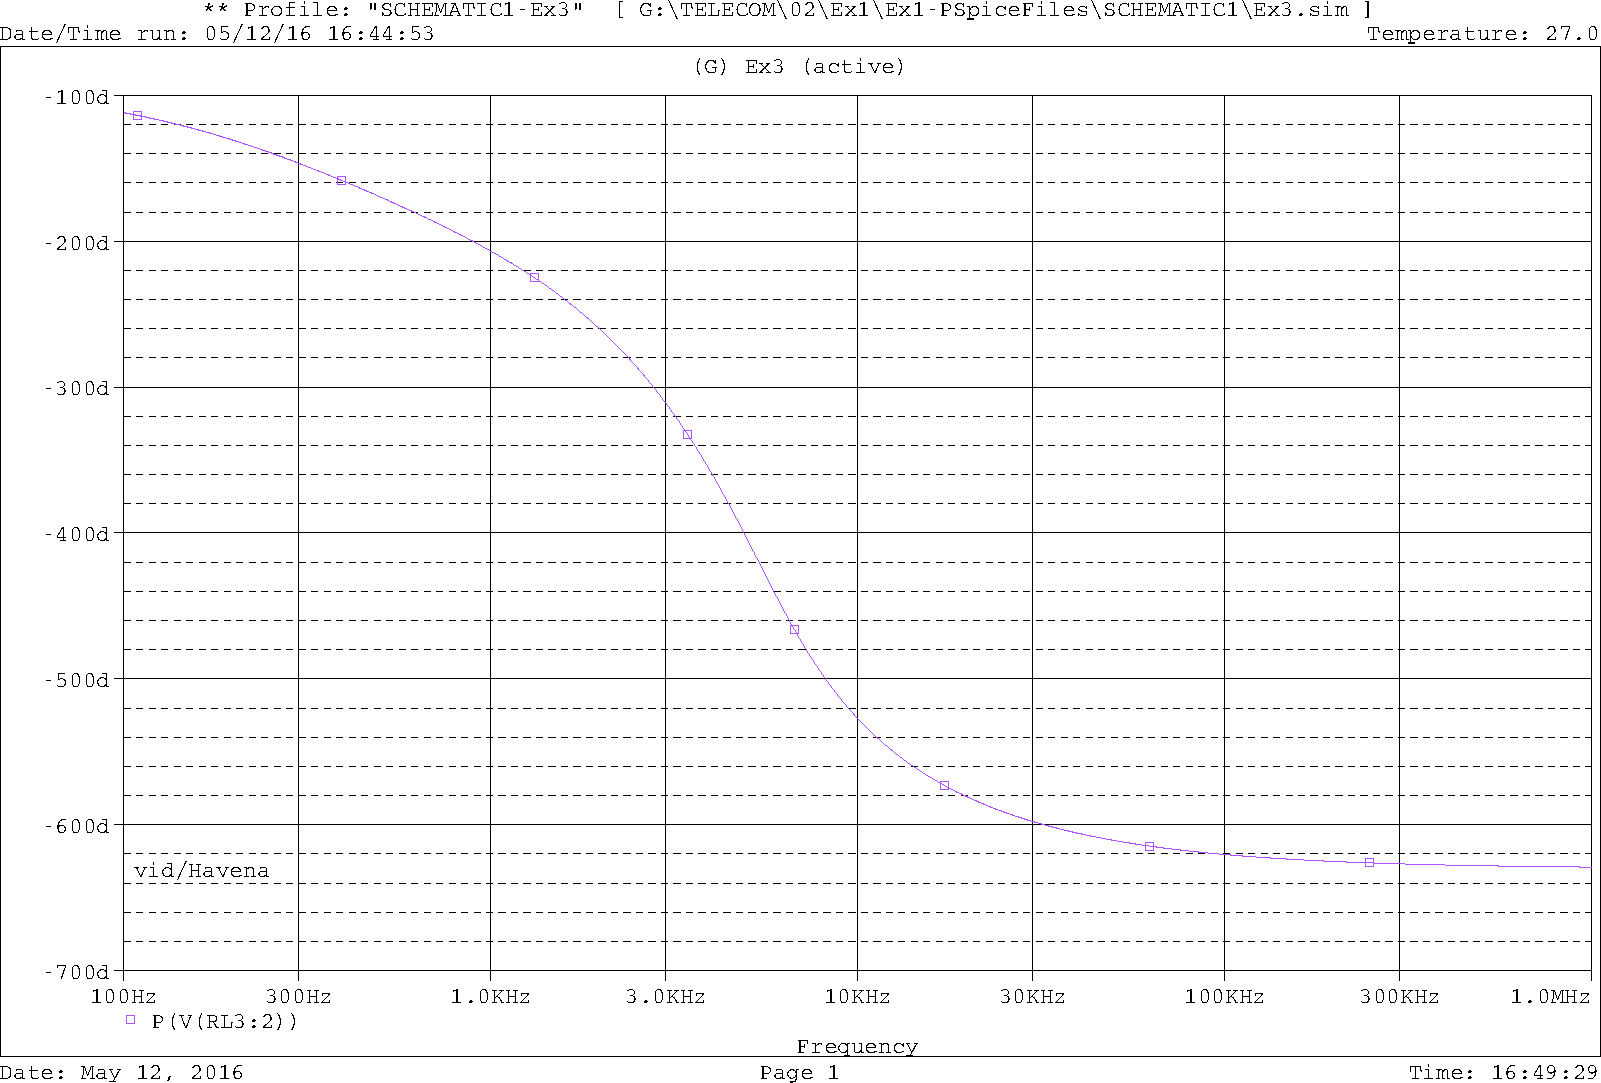
\includegraphics[scale=0.3]{Imagens/resp_freq_phase_3}
  \label{fig:resp_freq_phase_3}
  \caption{Fase da resposta em frequência do filtro passa-faixa em cascata.}
\end{figure}

\subsection{FPF}
O quarto e ultimo filtro foi projetado para ter uma resposta em frequência 
semelhante a do filtro FPF. O objetivo foi de analisar as diferenças 
em se utilizar um filtro FPF e um filtro FPB em conjunto com um filtro FPA.

O terceiro filtro projetado foi um filtro passa-faixas em cascata de terceira 
ordem, com resposta do tipo Butterworth utilizando apenas 1 indutor.

A figura \ref{fig:fpf} mostra o circuito já desnormalizado, pronto para 
simulação.

\begin{figure}[!h]
  \centering
  
  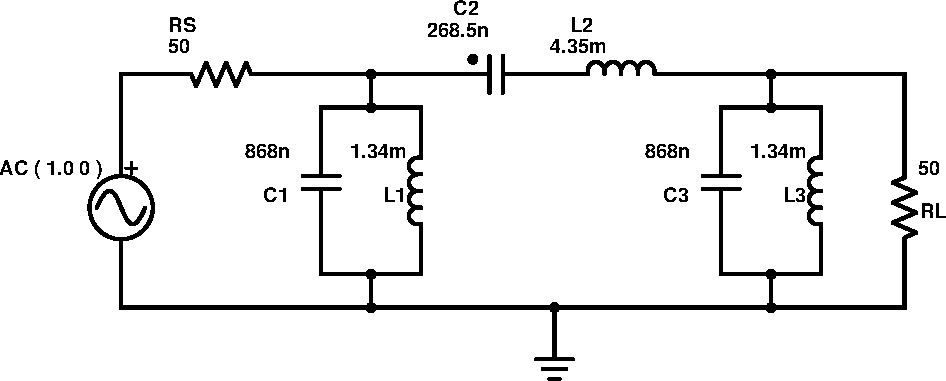
\includegraphics[scale=0.4]{Imagens/fpf}
  \label{fig:fpf}
  \caption{Filtro desnormalizado passa-faixa.}
\end{figure}

A resposta em frequência obtida está na figura \ref{fig:resp_freq_4}, onde foi 
obtido uma frequência central de 4,655 kHz. 

\begin{figure}[!h]
  \centering
  
  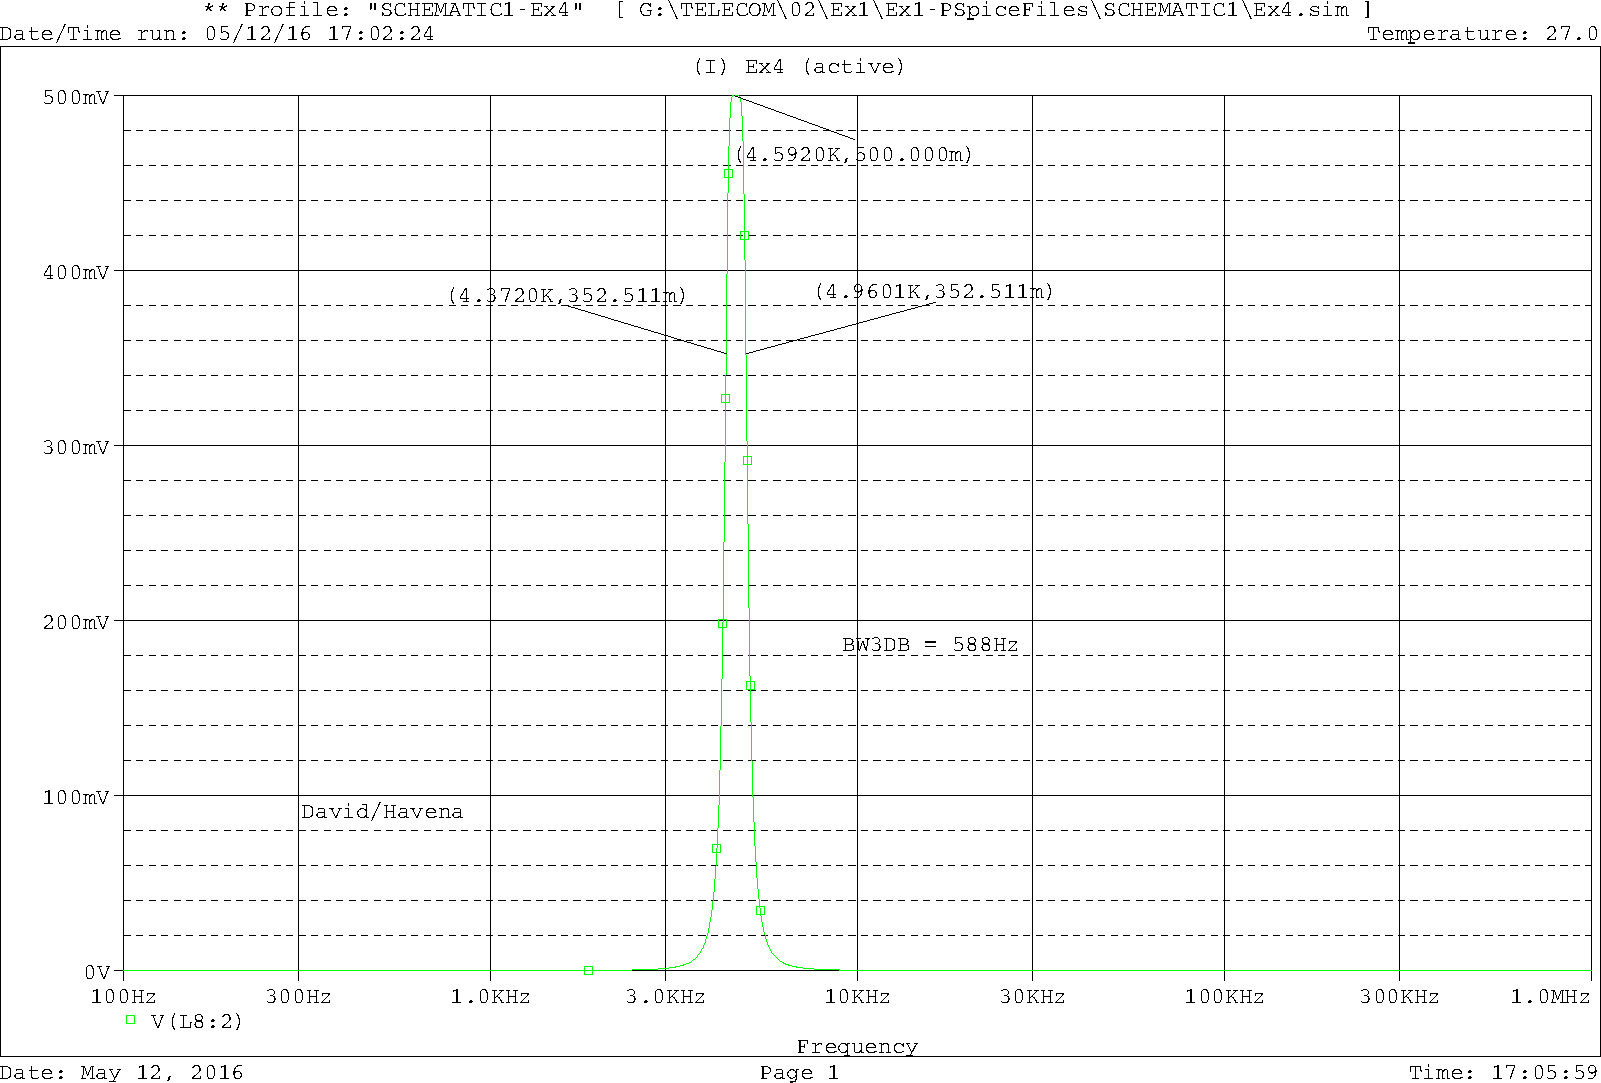
\includegraphics[scale=0.3]{Imagens/resp_freq_4}
  \label{fig:resp_freq_4}
  \caption{Resposta em frequência do filtro passa-faixa.}
\end{figure}

A figura \ref{fig:resp_freq_db_4} mostra a resposta em dB, nota-se que a 
atenuação aumenta em aproximadamente 60 dB por década, o que corresponde a 
ordem 3 do filtro.

\begin{figure}[!h]
  \centering
  
  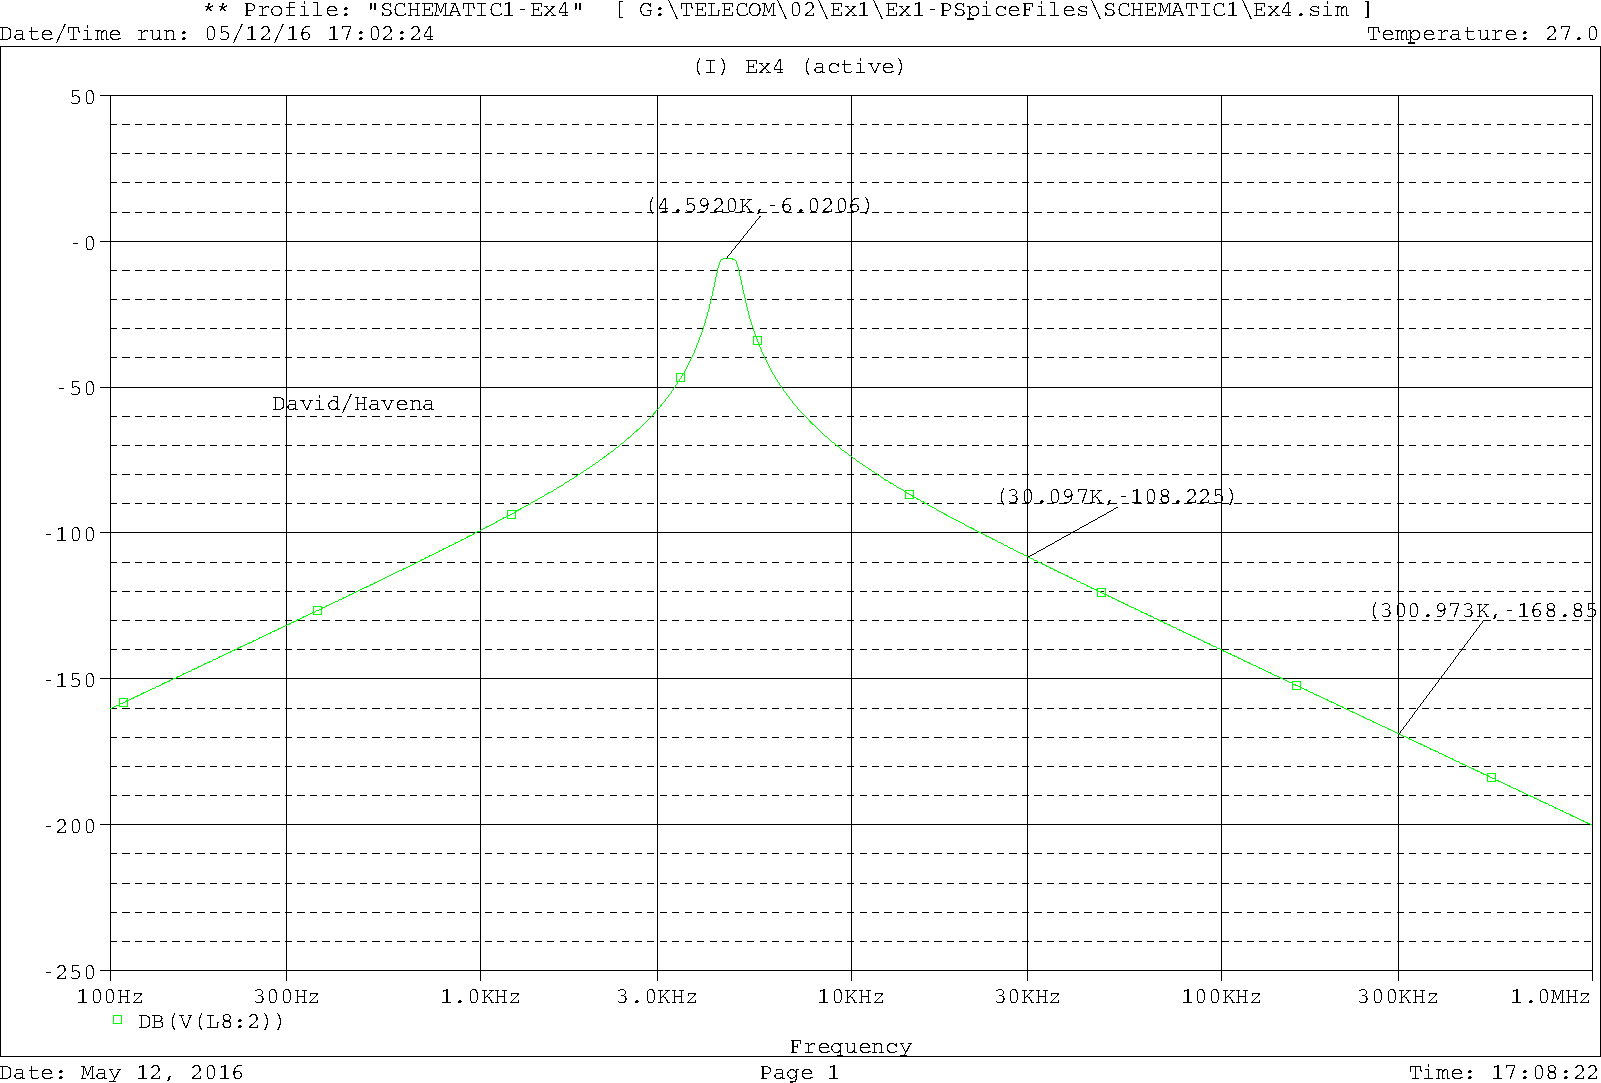
\includegraphics[scale=0.3]{Imagens/resp_freq_db_4}
  \label{fig:resp_freq_db_4}
  \caption{Resposta em frequência do filtro passa-faixa em dB.}
\end{figure}

A figura \ref{fig:resp_freq_phase_4} mostra a fase da resposta em frequência 
para o filtro passa altas, onde é possível observar uma defasagem de 270 graus, 
o que condiz com a teoria pois o filtro é de ordem 3.

\begin{figure}[!h]
  \centering
  
  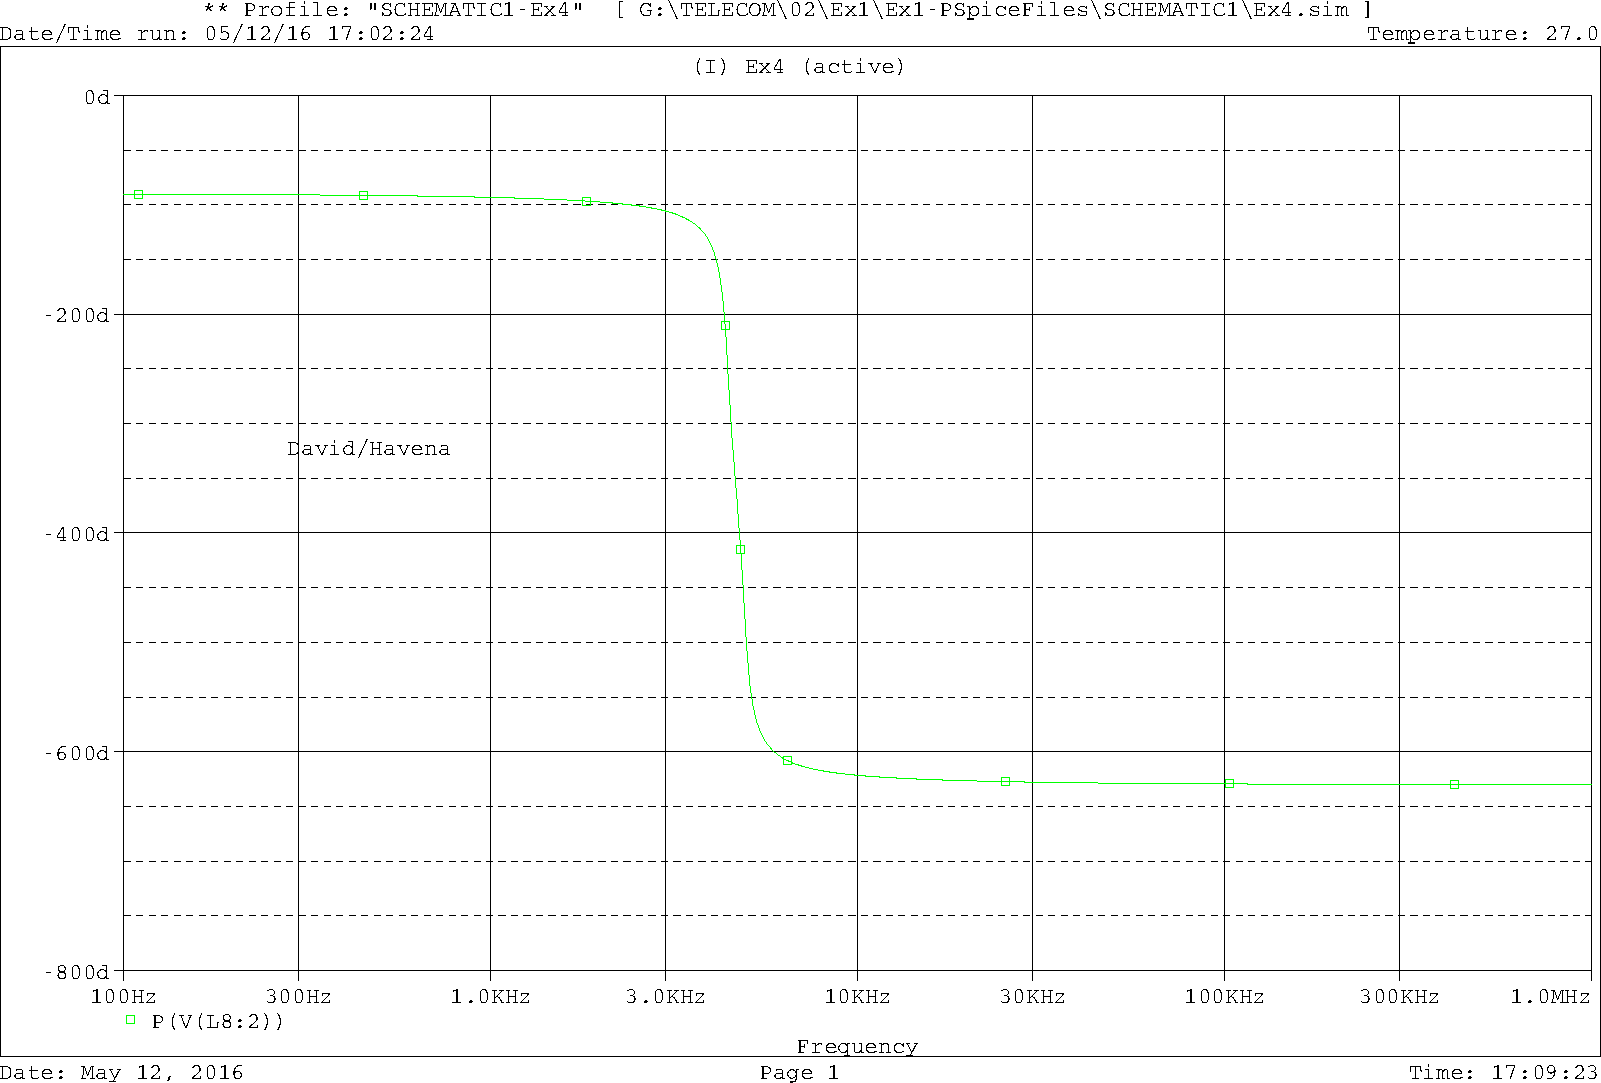
\includegraphics[scale=0.3]{Imagens/resp_freq_phase_4}
  \label{fig:resp_freq_phase_4}
  \caption{Fase da resposta em frequência do filtro passa-faixa.}
\end{figure}
\newpage
\section{Discussão e Conclusão}
Comente os resultados obtidos, sua qualidade e confiabilidade. Tente justificar eventuais discrepâncias que forem observadas. Aponte sugestões para melhorar a qualidade dos dados etc. Coloque as condições resultantes da experiência. Você deve discernir claramente quais foram essas conclusões. Não coloque como conclusões afirmações (mesmo que corretas) que não decorrem diretamente da experiência realizada. Se possível, relacione essas conclusões com as de outras experiências. Verifique até que ponto os objetivos da experiência foram alcançados (teste de um modelo, aplicações etc.).
\begin{thebibliography}{3}
\addcontentsline{toc}{section}{Referências}

\bibitem{malvino}
{\sc Malvino, A. P. Eletrônica. 4ª edição. Volume 1. MAKRON Books.}

\bibitem{sedra}
{\sc Sedra, A. S. Smith, K. C. Microeletrônica. 4ª edição. MAKRON Books.}


\end{thebibliography}


\end{document}